\chapter{Метод першого диференціального наближення}

\shortLectureDescription{Диперсійність та дисипативність різницевих рівнянь. Метод першого диференціального наближення. Приклади застосування методу диференціального наближення. Гіперболічна та параболічна форми запису першого диференціального наближення. Схемна в'язкість.}

\section{Метод першого диференціального наближення}

\emph{Метод першого диференціального наближення} є важливим інструментом дослідження різницевих схем. Згідно з цим методом усі функції дискретного аргументу, які входять до різницевого рівняння, розвиваються в ряди Тейлора. Ці розвинення підставляються в різницеве рівняння. У рівнянні залишають доданки, які залежать від кроків у нульовому та першому ступені, і аналізують якість одержаного рівняння, виходячи з відомих умов, що накладаються на коефіцієнти даного диференціального рівняння. Проведення такого аналізу пов'язано з тим, що виконання розрахунків на ЕОМ допускає використання хоча й досить малих, але все ж таки скінченних кроків сітки. Оцінки апроксимації мають асимптотичний  характер і не дають змоги отримати реальну оцінку похибки обчислень, яку необхідно враховувати, аналізуючи схему.

\begin{example}
    Ідею використання методу першого диференціального наближення проілюструємо на різницевій схемі Лакса 
    \begin{equation}
        \label{eq:l9.1}
        u_i^{n+1} = \frac{u_{i+1}^n+u_{i-1}^n}{2} -\frac{k\tau}{2h_x}(u_{i+1}^n-u_{i-1}^n),
    \end{equation}
    яка апроксимує хвильове диференціальне рівняння 
    \begin{equation}
        \label{eq:l9.2}
    	\frac{\partial u}{\partial t} = -k \frac{\partial u}{\partial x}.
    \end{equation}
\end{example}

Припускаючи, що розглядувана функція має достатню кількість неперервних похідних, розвинемо її в околі точки $(x_i,t_n)$ за формулою Тейлора за часовою
\begin{equation*}
    u_i^{n+1}=u_i^n+\tau\left.\frac{\partial u}{\partial t}\right|_i^n+\frac{\tau^2}{2}\left.\frac{\partial^2 u}{\partial t^2}\right|_i^n+O(\tau^3),
\end{equation*}
і просторовою змінними
\begin{equation*}
    u_{i\pm1}^n=u_i^n\pm h_x\left.\frac{\partial u}{\partial x}\right|_i^n+\frac{h_x^2}{2}\left.\frac{\partial^2 u}{\partial x^2}\right|_i^n\pm\frac{h_x^3}{6}\left.\frac{\partial^3 u}{\partial x^3}\right|_i^n+O(h^4),
\end{equation*}

Підставляючи ці розвинення в схему Лакса, дістанемо
\begin{equation*}
    0 = u_i^{n+1}-\frac{u_{i+1}^n+u_{i-1}^n}{2}+\frac{k\tau}{2h_x}(u_{i+1}^n-u_{i-1}^n)=\tau\frac{\partial u}{\partial t}+\tau k\frac{\partial u}{\partial x}+\frac{\tau^2}{2}\frac{\partial^2 u}{\partial t^2}-\frac{h_x^2}{2}\frac{\partial^2 u}{\partial x^2}+O(h_x^2+\tau^3).
\end{equation*}

Звідси маємо 
\begin{equation*}
    \frac{\partial u}{\partial t}=-k\frac{\partial u}{\partial x}-\frac{\tau}{2}\frac{\partial^2 u}{\partial t^2}+\frac{h_x^2}{2\tau}\frac{\partial^2 u}{\partial x^2}+O(h_x^2+\tau^2).
\end{equation*}

Це \textbf{гіперболічна форма} подання першого диференціального наближення. Продиференціювавши рівняння \eqref{eq:l9.2} за часом: 
\begin{equation*}
    \frac{\partial}{\partial t} \frac{\partial u}{\partial t} = \frac{\partial}{\partial t} \left(-k\frac{\partial u}{\partial x}\right)=\frac{\partial}{\partial x}\left(-k\frac{\partial u}{\partial t}\right)
\end{equation*} 
і підставивши в нього замість $\frac{\partial u}{\partial t}$ праву частину рівняння $-k\frac{\partial u}{\partial x}$, дістанемо
\begin{equation*}
    \frac{\partial^2 u}{\partial t^2} = \frac{\partial}{\partial x}\left(-k\left(-k\frac{\partial u}{\partial x}\right)\right) = k^2\frac{\partial^2 u}{\partial x^2}.
\end{equation*} 

Отже, перше диференціальне наближення можна подати у параболічній формі
\begin{equation*}
    \frac{\partial u}{\partial t}=-\frac{\partial u}{\partial x}+\left(\frac{h_x^2}{2\tau}-\frac{\tau k^2}{2}\right) \frac{\partial^2 u}{\partial x^2}+O(h_x^2+\tau^2).
\end{equation*}

Якщо $h_x \to 0$ і $\tau \to 0$, це рівняння перетворюється на початкове. Але оскільки розрахунки виконуються хоча при малих, але все ж таки скінченних кроках сітки $\tau > 0$, то при дослідженні доцільно залишати в апроксимуючому рівнянні принаймні перше наближення розвинення. Це вказує на те, що схема Лакса еквівалентна рівнянню дифузії
\begin{equation}
    \label{eq:l9.3}
    \frac{\partial u}{\partial t}=-\frac{\partial u}{\partial x}+\alpha\frac{\partial^2 u}{\partial x^2}
\end{equation}
з ефективною схемною дифузією $\alpha = \frac{h_x^2}{2\tau}-\frac{\tau k^2}{2}$, яка відсутня у вхідному рівнянні. При досить малих значення кроку за часом коефіцієнт штучної дифузії буде значним, а отже і достатнім для стабілізації розрахунків з потужними ударними хвилями. Якщо $C = 1$, демпфування зникає і таку схему не доцільно використовувати для розрахунку ударних хвиль. \medskip

Для коректності задачі в рівнянні переносу коефіцієнт дифузії має бути додатним, тобто 
\begin{equation}
	\label{eq:l9.4}
    \alpha = \frac{h_x^2}{2\tau}-\frac{\tau k^2}{2}\ge0.
\end{equation}

Це можливо при $h^2-k^2\tau^2\ge0$. Звідси встановлюємо, що умовою стійкості схеми Лакса буде $|C|\le1$, а при $C=1$ схема Лакса дає точний розв'язок модельного рівняння (де $C=\frac{k\tau}{h}$ --- число Куранта). \medskip

З першого диференціального наближення випливає, що похибка апроксимації схеми Лакса дорівнює $O(\tau,h_x^2,h_x^2/\tau)$. Отже, схема апроксимує диференціальне рівняння тільки тоді, коли прямують до нуля одночасно кроки сітки $\tau$ та $h_x$ і відношення $h_x^2\tau$.

\begin{remark}
    До недоліків схеми Лакса відносять погану її пристосованість до роз\-в'я\-зу\-ван\-ня задач дозвукових і безударних потоків. Вона не задовольняє вимоги транспортивності, тобто дозволяє розповсюджувати малі збурення проти потоку надзвукового не в'язкого газу.
\end{remark}

Останнє твердження легко перевірити. Для цього достатньо розглянути схему передавання інформації з $n$-го часового кроку на $(n+1)$-й. Так, при переході до вузла $(x_i,t_{n+1})$ використовується інформація, яка міститься у вузлах $(x_{i-1},t_n)$ і $(x_{i+1},t_n)$. Отже, при будь-якому напрямі вектора швидкості потоку довільне мале збурення має змогу передаватися в протилежному до нього напрямі. \medskip

Незважаючи на зазначені недоліки, схема Лакса має важливу перевагу --- простоту реалізації. Крім того, вона легко адаптується як до циліндричних, так і до сферичних систем координат. \medskip

\begin{example}
    Застосуємо метод першого диференціального наближення до дослідження різницевої схеми для рівняння переносу
    \begin{equation}
        \label{eq:l9.5}
        \frac{\partial u}{\partial t} = -k\frac{\partial u}{\partial x} + \alpha \frac{\partial^2 u}{\partial x^2},
    \end{equation}
    для якого явна схема має вигляд
    \begin{equation*}
        \frac{u_i^{n+1}-u_i^n}{\tau}=-2k\frac{u_{i+1}^n-u_{i-1}^n}{h}+\alpha\frac{u_{i+1}^n-2u_i^n+u_{i-1}^n}{h^2}.
    \end{equation*}
\end{example}

Записавши для членів $u_i^{n+1}$, $u_{i\pm1}^n$ формули Тейлора в околі точки  
\begin{equation*}
    u_i^{n+1}=u_i^n+\tau\left.\frac{\partial u}{\partial t}\right|_i^n+\frac{\tau^2}{2}\left.\frac{\partial^2 u}{\partial t^2}\right|_i^n+O(\tau^3),
\end{equation*}
\begin{equation*}
    u_{i\pm1}^n=u_i^n\pm h\left.\frac{\partial u}{\partial x}\right|_i^n+\frac{h^2}{2}\left.\frac{\partial^2 u}{\partial x^2}\right|_i^n\pm\frac{h^3}{6}\left.\frac{\partial^3 u}{\partial x^3}\right|_i^n+O(h^4),
\end{equation*}
і підставивши їх у різницеву схему, дістанемо рівняння
\begin{equation*}
    \frac{\partial u}{\partial t} + \frac{\tau}{2} \frac{\partial^2 u}{\partial t^2} = -k \frac{\partial u}{\partial x} + \alpha \frac{\partial^2 u}{\partial x^2} + O(\tau^2, h^2).
\end{equation*}

Якщо $h \to 0$ і $\tau \to 0$, це рівняння перейде в рівняння переносу, але при $\tau > 0$, $h > 0$ його перше диференціальне наближення є гіперболічним рівнянням
\begin{equation}
    \label{eq:l9.6}
    \frac{\tau}{2\alpha} \frac{\partial^2 u}{\partial t^2} - \frac{\partial^2 u}{\partial x^2} + \frac{1}{\alpha} \frac{\partial u}{\partial t} + \frac{k}{\alpha} \frac{\partial u}{\partial x} = 0.
\end{equation}

Отримане рівняння має область впливу довільної точки $(x,t)$, обмежену характеристиками з тангенсами кута нахилу $\pm\sqrt{\frac{\tau}{2\alpha}}$. Збурення, які виникають у точці $(x,t)$, мають вплив лише всередині зазначеної області. \medskip

Для різницевої схеми також існує область впливу. Оскільки кожне значення $u_i^{n+1}$ залежить від $u_{i\pm1}^n$, то область впливу сіткового рівняння обмежується лініями з тангенсами кутів нахилу $\pm\tau/h$. Умова стійкості для таких рівнянь вимагає, щоб область впливу різницевого рівняння принаймні вміщувала область впливу диференціального рівняння. Тобто $\frac{\tau}{h} \le \sqrt{\frac{\tau}{2\alpha}}$. Звідси маємо таку умову стійкості різницевої схеми
\begin{equation}
    \label{eq:l9.7}
    \tau \le \frac{h^2}{2\alpha}.
\end{equation}

Параболічна форма запису першого диференціального наближення визначає другу необхідну умову стійкості. \medskip

Для побудови параболічної форми першого диференціального наближення визначимо $\frac{\partial^2 u}{\partial t^2}$. Продиференціювавши рівняння переносу \eqref{eq:l9.5} за часом і використавши саме рівняння, маємо:
\begin{equation*}
    \frac{\partial^2 u}{\partial t^2} = k^2 \frac{\partial^2 u}{\partial x^2} - 2 k \alpha \frac{\partial^3 u}{\partial x^3} + \alpha^2 \frac{\partial^4 u}{\partial x^4}.
\end{equation*}

Підставимо цю рівність в початкове рівняння. Після простих перетворень і відкидання членів з похідними третього і четвертого порядків маємо
\begin{equation}
    \label{eq:l9.8}
    \frac{\partial u}{\partial t} = -k \frac{\partial u}{\partial x} + \alpha \frac{\partial^2 u}{\partial x^2},
\end{equation}
де $\alpha = \alpha - \frac{k^2 \tau}{2}$.  \medskip

Нехтування членами з похідними порядків вищих другого обґрунтовується тим, що, по-перше, їх величини значно менші за решту похідних; по-друге, a posteriori відомо, що умова стійкості, отримана в результаті цього аналізу, дасть жорсткіші обмеження на крок за часом у присутності дифузійного члена лише для течій з малою в'язкістю, тобто для $\alpha \ll k$, коли коефіцієнти при старших похідних у рівнянні стають малими. \medskip

Оскільки коректність постановки задачі вимагає, щоб в'язкість була невід'ємною, то друга умова стійкості має вигляд  $\tau \le \frac{2\alpha}{k^2}$.

\begin{example}
    Явні однокрокові двошарові схеми з різницями проти потоку для розв'язування хвильового рівняння можна подати у вигляді
    \begin{equation}
        \label{eq:l9.9}
        \frac{u_i^{n+1} - u_i^n}{\tau} = \begin{cases}
            -k \frac{u_i^n - u_{i-1}^n}{h}, & k > 0, \\
            -k \frac{u_{i+1}^n - u_i^n}{h}, & k < 0.
        \end{cases}
    \end{equation}
\end{example}

Якщо $C = 1$, ця схема дає точний розв'язок хвильового рівняння. Ця умова є також і граничною умовою стійкості. Дослідження стійкості за методом фон Неймана показує, що при $|C| < 1$, де $C = \frac{k\tau}{h}$ --- число Куранта, коефіцієнт переходу (чи норма матриці для системи рівнянь) буде меншим від одиниці. Будь-яка схема для рівняння лише з одним конвективним доданком при $C < 1$  має схемне загасання. \medskip

Використання першого диференціального наближення показує, що при врахуванні членів, у які входять кроки сітки в першому ступені, це рівняння еквівалентне рівнянню повного переносу
\begin{equation*}
    \frac{\partial u}{\partial t} = -\frac{\partial (cu)}{\partial x} + \alpha_c \frac{\partial^2 u}{\partial x^2} + o(\Delta x^2)
\end{equation*}
з не фізичною в'язкістю $\alpha_c = 0.5 k h (1 - C)$. Це пояснює не лише наявність штучного загасання, а й те, що схема з різницями проти потоку має штучну дифузію (штучну в'язкість). Інтерпретація цього факту в багатовимірному випадку, а також для в'язких течій не така очевидна. \medskip

Дослідження випадку, коли $k < 0$, проводиться аналогічно і приводять до тих же, що раніше одержано умов стійкості. різницевої схеми.

\section{Штучна в'язкість. Дисипація та дисперсія різницевих схем}

Як було показано у попередньому пункті, при $|C| \ne 1$ схема з різницями проти потоку має \emph{схемну в'язкість} $\alpha = \frac{k^2 \tau}{2} > 0$.

\begin{definition}
    Таку в'язкість називають також \emph{штучною в'язкістю}.
\end{definition}

Ця в'язкість на відміну від явної, яку у різницеве рівняння уводять цілеспрямовано, є внутрішньою характеристикою різницевої задачі. Схемна в'язкість згладжує розривні розв'язки рівняння, зменшує градієнти всіх параметрів незалежно від причини виникнення цих градієнтів, фізичної чи обчислювальної. 

\begin{definition}
    Така властивість різницевої схеми, обумовлена присутністю у виразі для похибки апроксимації похідних парного порядку за просторовою змінною називається \emph{дисипацією} на різницевій сітці.
\end{definition}

Дисипація здебільше визначає відносну похибку обчислення амплітуди розв'язку.

\begin{definition}
    Друга близька за фізичним змістом властивість різницевої схеми є \emph{дисперсія}.
\end{definition}

Вона безпосередньо пов'язана з похідними непарного порядку за просторовими змінними у виразі для похибки апроксимації. Дисперсія приводить до невірного відображення відношення фаз різних хвиль. \medskip

Дисперсія визначає внесок у розв'язок похибки визначення фази розв'язку.

\begin{definition}
    Сумісна дія дисперсії та дисипації на розв'язок у ряді випадків називають \emph{дифузією}.
\end{definition}

Дифузія приводить до розтягу крутих ліній розділу, які можуть виникати у області розрахунку. \medskip

Так, чисельний розв'язок, одержаний у тому випадку, коли похибка в основному є дисипативною (такий розв'язок типовий для схем першого порядку точності), значно згладжує лінії великих градієнтів. Подібні схеми не доцільно використовувати для розрахунків, які повинні досить точно відображати рух розривів. Разом з тим вони можуть бути корисними при знаходженні стаціонарного розв'язку.\medskip

Чисельні розв'язки, які одержані у випадку коли схема є дисперсійною (це притаманно для схем другого порядку точності) вносять нефізичні коливання (осциляції) розв'язку навіть при незначних збуреннях. Ці коливання з'являються перед і після точки виникнення збурення. Здебільше такі схеми використовуються для знаходження гладких розв'язків. \medskip

Дослідження похибок розв'язків різницевих рівнянь можна проводити за допомогою аналізу модуля та аргументу коефіцієнту переходу. Запишемо коефіцієнт переходу для схеми  
\begin{equation*}
    \frac{u_i^{n+1}-u_i^n}{\tau}=\frac{(ku)_i^n-(ku)_{i-1}^n}{h}
\end{equation*}
для рівняння
\begin{equation*}
    \frac{\partial u}{\partial t} = -\frac{\partial (k u)}{\partial x}, \quad k > 0
\end{equation*}
у вигляді
\begin{equation*}
    G = (1 - C + C \cos \beta) - I (C \sin \beta)
\end{equation*}
або
\begin{equation*}
    G = |G| e^{I\phi},
\end{equation*}
де 
\begin{equation*}
    |G| = \sqrt{(1-C+C\cos\beta)^2+(C\sin\beta)^2},
\end{equation*}
\begin{equation*}
    \phi = \arg G = \arctan \frac{\Imag G}{\Real G} = \arctan \left( \frac{-C\sin\beta}{1-C+C\cos\beta}\right)
\end{equation*}
а $\beta=mh$ --- хвильове число.

\begin{definition}
	\emph{Фазовий кут} точного аналітичного розв'язку хвильового рівняння $\phi_e$ визначається аналогічно, через відомий коефіцієнт переходу точного розв'язку хвильового рівняння.
\end{definition}

Для визначення точного значення коефіцієнта переходу підставимо у хвильове рівняння його фундаментальний розв'язок $u = e^{\alpha t}e^{Ik_mx}$ і знайдемо, що $\alpha=-Ik_mk$. Тоді $u=e^{Ik_m(x-kt)}$, а отже, коефіцієнт переходу для точного розв'язку має вигляд
\begin{equation*}
    G_e = \frac{u(t + \Delta t)}{u(t)} = \frac{e^{Ik_m(x-k(t+\Delta t))}}{e^{Ik_m(x-kt))}}.
\end{equation*}

З останнього співвідношення випливає, що
\begin{equation*}
    G_e = e^{-Ik_mk\Delta t}=e^{I\phi_e}.
\end{equation*}

Тобто $|G|=1$, а $\phi_e=-k_mk\Delta t=-\beta C$. 

\begin{proposition}
    Отже, \emph{сумарна похибка у визначенні амплітуди}, яка обумовлена дисипацією, після $n$ часових кроків розв'язку хвильового рівняння з різницями проти потоку рівна 
    \begin{equation*}
        (1 - |G|^n) A_0,
    \end{equation*}
    де $A_0$ --- початкове значення амплітуди хвилі. 
\end{proposition}

\begin{proposition}
    Аналогічно можна визначити \emph{дисперсійну} похибку (викривлення фази хвилі) як $n (\phi_e - \phi)$. 
\end{proposition}

\begin{proposition}
    \emph{Відносна похибка} у визначенні зміщення за фазою на одному кроці за часом рівна
    \begin{equation*}
        \frac{\phi}{\phi_e} = \frac{\arctan \left( \frac{-C\sin\beta}{1-C+C\cos\beta}\right)}{-\beta C}
    \end{equation*}
\end{proposition}
 
При малих значення хвильових чисел $\beta$ вираз для відносної похибки при визначенні фази можна привести до вигляду
\begin{equation*}
    \frac{\phi}{\phi_e} \approx 1 - \frac{2C^2-3C+1}{6} \beta^2.
\end{equation*}

Якщо відносна похибка у визначенні фази при заданому $\beta$ більша від одиниці, то розрахункове значення швидкості розповсюдження відповідної гармонічної хвилі виявляється більшим від точного значення швидкості цієї хвилі. Такі хвилі розповсюджуються з \emph{випередженням за фазою}. \medskip

Аналогічно, якщо відносна похибка у визначенні фази менша від одиниці, то розрахункова швидкість розповсюдженні гармонічної хвилі виявляється меншою від точного значення швидкості цієї хвилі, тому кажуть, що такі хвилі розповсюджуються з \emph{відставанням за фазою}. \medskip

При використовуванні різницевої схеми з різницями проти потоку випередження за фазою виникає при $\half < C < 1$, а відставання при $C < \half$. \medskip

Розглядаючи неявний метод Ейлера, приходимо до висновку, що його перше диференціальне наближення має вигляд
\begin{equation*}
    \frac{\partial u}{\partial t} + k \frac{\partial u}{\partial x} = \frac{k^2 \Delta t}{2} \frac{\partial^2 u}{\partial x^2},
\end{equation*}
а коефіцієнт переходу та відносна похибка визначення фази записуються відповідно так
\begin{equation*}
    G = \frac{1 - I C \sin \beta}{1 + C^2 \sin^2 \beta},
\end{equation*}
та
\begin{equation*}
    \frac{\phi}{\phi_e} = \frac{\arctan(- C \sin \beta)}{-\beta C}.
\end{equation*}

Неявний метод Ейлера веде до значної дисипації при середніх хвильових числах і до значного запізнення за фазою при великих хвильових числах.

\section{Приклади проявлення штучної в'язкості, дифузії}

\subsection{Двокроковий симетризований алгоритм (ДС-алгоритм)}

Розв'язки задачі про рух квадратної хвилі за допомогою алгоритму (2.37)--(2.40) на 200 кроці відповідно
\begin{figure}[H]
    \centering
    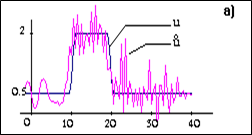
\includegraphics{{img/10/5.3.a}.png}
    \label{fig:5.3.a}
    \caption{без штучної в'язкості ($\alpha = 1$, $\beta=-1$, $\sigma=0.01$, $\sigma_1=0$, $\sigma_3=0$, $\sigma_2=0$; $h=0.5$, $\tau=0.25$)}
\end{figure}
\begin{figure}[H]
    \centering
    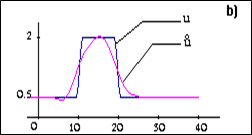
\includegraphics{{img/10/5.3.b}.png}
    \label{fig:5.3.b}
    \caption{із штучною в'язкістю ($\alpha = 1$, $\beta=-1$, $\sigma=0.01$, $\sigma_1=0.1$, $\sigma_3=0.1$, $\sigma_2=0$; $h=0.5$, $\tau=0.25$)}
\end{figure}
\begin{figure}[H]
    \centering
    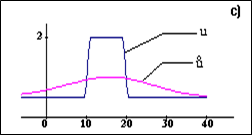
\includegraphics{{img/10/5.3.c}.png}
    \label{fig:5.3.c}
    \caption{із надто великою штучною в'язкістю ($\alpha = 1$, $\beta=-1$, $\sigma=0.01$, $\sigma_1=0.1$, $\sigma_3=0.1$, $\sigma_2=0$; $h=0.5$, $\tau=0.25$)}
\end{figure}

Тут і далі $u$ --- точний розв'язок, $\overset{\circ}{u}$ --- розв'язок, знайдений за допомогою ДС-методу (2.37), (2.38). На наступних малюнках представлені результати тестування ДС-алгоритмів із штучною в'язкістю ($a$ --- коефіцієнт при явній штучній в'язкості, $a_1$ --- коефіцієнт при неявній штучній в'язкості) на вказаних модельних задачах (схеми, в яких явні частини --- проти потоку, неявні частини --- за потоком).

\begin{minipage}[t]{.45\textwidth}
    \begin{figure}[H]
        \centering
        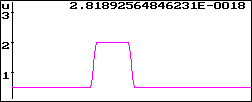
\includegraphics{{img/10/5.4}.png}
        \label{fig:5.4}
        \caption{\scriptsize $h=0.5$, $\tau=0.5$, $\sigma=2$, $a=0$, $a_1=0$}
    \end{figure}
\end{minipage}
\begin{minipage}[t]{.45\textwidth}
    \begin{figure}[H]
        \centering
        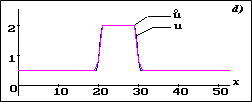
\includegraphics{{img/10/5.5}.png}
        \label{fig:5.5}
        \caption{\scriptsize $h=0.5$, $\tau=0.5$, $\sigma=0.01$, $a=0$, $a_1=0$}
    \end{figure}
\end{minipage}

\begin{minipage}[t]{.45\textwidth}
    \begin{figure}[H]
        \centering
        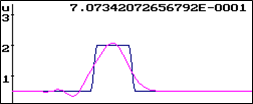
\includegraphics{{img/10/5.6}.png}
        \label{fig:5.6}
        \caption{\scriptsize $h=0.5$, $\tau=0.25$, $\sigma=1$, $a=1$, $a_1=1$}
    \end{figure}
\end{minipage}
\begin{minipage}[t]{.45\textwidth}
    \begin{figure}[H]
        \centering
        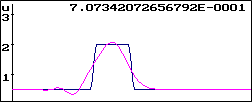
\includegraphics{{img/10/5.7}.png}
        \label{fig:5.7}
        \caption{\scriptsize $h=0.5$, $\tau=0.25$, $\sigma=0.01$, $a=0.1$, $a_1=0$}
    \end{figure}
\end{minipage}

\begin{minipage}[t]{.45\textwidth}
    \begin{figure}[H]
        \centering
        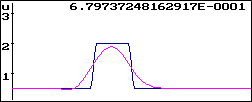
\includegraphics{{img/10/5.8}.png}
        \label{fig:5.8}
        \caption{\scriptsize $h=0.5$, $\tau=0.25$, $\sigma=0.01$, $a=0.1$, $a_1=0.1$}
    \end{figure}
\end{minipage}
\begin{minipage}[t]{.45\textwidth}
    \begin{figure}[H]
        \centering
        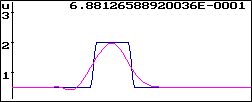
\includegraphics{{img/10/5.9}.png}
        \label{fig:5.9}
        \caption{\scriptsize $h=0.5$, $\tau=0.25$, $\sigma=0.01$, $a=0.1$, $a_1=0.05$}
    \end{figure}
\end{minipage}

\begin{minipage}[t]{.45\textwidth}
    \begin{figure}[H]
        \centering
        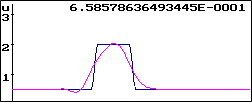
\includegraphics{{img/10/5.10}.png}
        \label{fig:5.10}
        \caption{\scriptsize $h=0.5$, $\tau=0.125$, $\sigma=0.01$, $a=0.5$, $a_1=0$}
    \end{figure}
\end{minipage}
\begin{minipage}[t]{.45\textwidth}
    \begin{figure}[H]
        \centering
        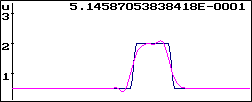
\includegraphics{{img/10/5.11}.png}
        \label{fig:5.11}
        \caption{\scriptsize $h=0.5$, $\tau=0.025$, $\sigma=0.01$, $a=2$, $a_1=2$}
    \end{figure}
\end{minipage}

\begin{minipage}[t]{.45\textwidth}
    \begin{figure}[H]
        \centering
        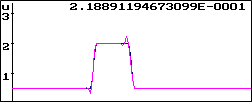
\includegraphics{{img/10/5.12}.png}
        \label{fig:5.12}
        \caption{\scriptsize $h=0.5$, $\tau=0.5$, $\sigma=100$, $a=1$, $a_1=0$}
    \end{figure}
\end{minipage}
\begin{minipage}[t]{.45\textwidth}
    \begin{figure}[H]
        \centering
        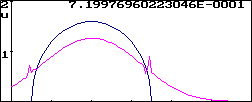
\includegraphics{{img/10/5.13}.png}
        \label{fig:5.13}
        \caption{\scriptsize $h=0.5$, $\tau=0.25$, $\sigma=1$, $a=1$, $a_1=1$}
    \end{figure}
\end{minipage}

\begin{minipage}[t]{.45\textwidth}
    \begin{figure}[H]
        \centering
        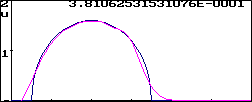
\includegraphics{{img/10/5.14}.png}
        \label{fig:5.14}
        \caption{\scriptsize $h=0.5$, $\tau=0.25$, $\sigma=0.01$, $a=0.1$, $a_1=0$}
    \end{figure}
\end{minipage}
\begin{minipage}[t]{.45\textwidth}
    \begin{figure}[H]
        \centering
        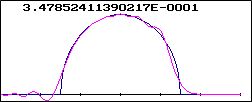
\includegraphics{{img/10/5.15}.png}
        \label{fig:5.15}
        \caption{\scriptsize $h=0.5$, $\tau=0.125$, $\sigma=0.01$, $a=0.1$, $a_1=0.05$}
    \end{figure}
\end{minipage}

\begin{minipage}[t]{.45\textwidth}
    \begin{figure}[H]
        \centering
        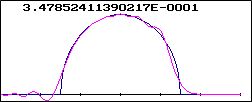
\includegraphics{{img/10/5.16}.png}
        \label{fig:5.16}
        \caption{\scriptsize $h=0.5$, $\tau=0.025$, $\sigma=0.01$, $a=0$, $a_1=0$}
    \end{figure}
\end{minipage}
\begin{minipage}[t]{.45\textwidth}
    \begin{figure}[H]
        \centering
        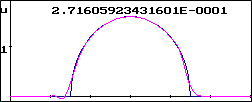
\includegraphics{{img/10/5.17}.png}
        \label{fig:5.17}
        \caption{\scriptsize $h=0.5$, $\tau=0.025$, $\sigma=0.01$, $a=2$, $a_1=2$}
    \end{figure}
\end{minipage}

\begin{minipage}[t]{.45\textwidth}
    \begin{figure}[H]
        \centering
        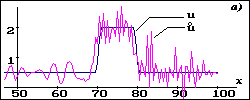
\includegraphics{{img/10/5.18}.png}
        \label{fig:5.18}
    \end{figure}
\end{minipage}
\begin{minipage}[t]{.45\textwidth}
    \begin{figure}[H]
        \centering
        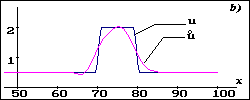
\includegraphics{{img/10/5.18.a}.png}
        \label{fig:5.18.a}
    \end{figure}
\end{minipage}

\begin{minipage}[t]{.45\textwidth}
    \begin{figure}[H]
        \centering
        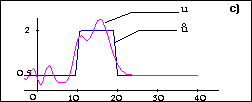
\includegraphics{{img/10/5.18.b}.png}
        \label{fig:5.18.b}
    \end{figure}
\end{minipage}
\begin{minipage}[t]{.45\textwidth}
    \begin{figure}[H]
        \centering
        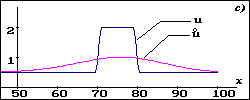
\includegraphics{{img/10/5.18.c}.png}
        \label{fig:5.18.c}
    \end{figure}
\end{minipage}

\begin{minipage}[t]{.3\textwidth}
    \begin{figure}[H]
        \centering
        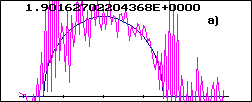
\includegraphics[width=\textwidth]{{img/10/5.19.a}.png}
        \label{fig:5.19.a}
    \end{figure}
\end{minipage}
\begin{minipage}[t]{.3\textwidth}
    \begin{figure}[H]
        \centering
        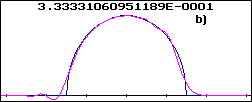
\includegraphics[width=\textwidth]{{img/10/5.19.b}.png}
        \label{fig:5.19.b}
    \end{figure}
\end{minipage}
\begin{minipage}[t]{.3\textwidth}
    \begin{figure}[H]
        \centering
        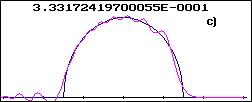
\includegraphics[width=\textwidth]{{img/10/5.19.c}.png}
        \label{fig:5.19.c}
    \end{figure}
\end{minipage}

\section{Завдання для самостійної роботи}

\shortHomeworkDescription{Дослідити перше диференціальне наближення телеграфного рівняння. Встановити наявність схемної в'язкості.}
